\documentclass[12pt]{article}
\usepackage{amsmath}
\usepackage{amssymb} %mathbb
\usepackage{graphicx}
\usepackage{hyperref}
\usepackage[latin1]{inputenc}
\usepackage[top=1.0cm,bottom=1.3cm,left=1.0cm,right=1.0cm]{geometry}

\begin{document}

		\begin{center}
		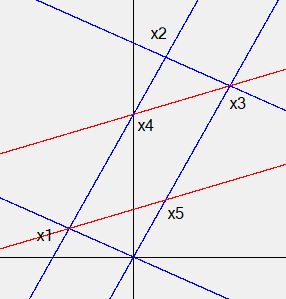
\includegraphics{restrita}
		\end{center}

\begin{align}
y_1 &= ax \text{ // passa pela origem, inclina\c{c}\~ao qualquer, perpendicular seria trivial.} \\
y_2 &= ax + b \text{ // vamos construir ret\^angulo. reta paralela qualquer.} \\
y_3 &= -\cfrac{x}{a} \text{ // perpendicular \`a primeira, passa pela origem.} \\
y_4 &= c - \cfrac{x}{a} \text{ // qualquer reta paralela \`a terceira.} \\
y_2 &= y_3 \Rightarrow a^2 x + ab = - x \Rightarrow x_1 = -\cfrac{ab}{a^2 + 1} \Rightarrow y(x_1) = ax_1 + b \\
y_2 &= y_4 \Rightarrow a^2 x + ab = ac - x \Rightarrow x_2 = \cfrac{ac - ab}{a^2 + 1} \Rightarrow y(x_2) = ax_2 + b \\
y_1 &= y_4 \Rightarrow a^2 x = ac - x \Rightarrow x_3 = \cfrac{ac}{a^2 + 1} \Rightarrow y(x_3) = ax_3 \\
z &= \cfrac{1}{a^2 + 1} \\
B &= \sqrt{x_3^2 + (ax_3)^2} = acz \sqrt{1 + a^2} \\
H &= \sqrt{x_1^2 + (-x_1/a)^2} = bz \sqrt{a^2 + 1} \Rightarrow S_1 = BH = abcz \text{ // Base vezes altura.} \\
S_2 &= \int_{x_1}^0 (y_2 - y_3) + \int_0^{x_2} (y_2 - y_1) + \int_{x_2}^{x_3} (y_4 - y_1) \text{ // dois tri\^angulos e um paralelogramo.} \\
S_2 &= \int_{x_1}^{x_2} (ax + b) + \int_{x_1}^0 (x/a) - \int_0^{x_3} (ax) + \int_{x_2}^{x_3} (c - x/a) \\
x_2 &= x_1 + x_3 \\
S_2 &= \cfrac{a(x_1 + x_3)^2 - ax_1^2}{2} + b(x_1 + x_3) - bx_1 - \cfrac{x_1^2}{2a} - \cfrac{ax_3^2}{2} + cx_3 - c(x_1 + x_3) + \cfrac{- x_3^2 + (x_1 + x_3)^2}{2a} \\
S_2 &= ax_1x_3 + bx_3 - cx_1 + \cfrac{x_1x_3}{a} = -a\cdot abz\cdot acz + b\cdot acz + cabz - \cfrac{abz\cdot acz}{a} \\
S_2 &= abcz (-a^2z + 2 - z) = abcz \therefore S_2 = S_1
\end{align}

\vspace{100mm}

Agora com velocidade na dire\c{c}\~ao de $u = \tan \theta$.

\begin{align}
\beta &= \text{dist}(p_3, p_4) \\
S_1 &= \cfrac{\beta h_1}{2} + \beta h_2 + \cfrac{\beta h_1}{2} = abcz \text{ // velocidade zero, tri\^angulos congruentes.} \\
\gamma &= \sqrt{1 - \cfrac{v^2}{c^2}} \in (0, 1]\text{, porque }v < c\text{ // constante de contra\c{c}\~ao.} \\
\beta(v) &= \beta\gamma \text{ // a altura se mant\'em constante.} \\
S_3(v) &= \cfrac{\beta\gamma h_1}{2} + \beta\gamma h_2 + \cfrac{\beta\gamma h_1}{2} = abcz\gamma \\
\therefore S_3(v) &= \gamma S_1 = \gamma\cdot S_3(0)
\end{align}

Est\'a provado que a \'area s\'o muda se variar o m\'odulo da velocidade: $S_f \ne S_0 \Leftrightarrow \Vert v_f\Vert \ne \Vert v_0\Vert$.

\end{document}
